\chapter{Concept 1: Unity Machine Learning Agents}
\lhead{\thechapter \space Concept 1: Unity Machine Learning Agents}
\label{ch:concept_one}
The first concept chosen was the \gls{mlagents} approach mentioned in section \ref{sec:approach_ml_agents}. This chapter describes the concept of this approach, the reasons for choosing this approach over the others, the simulation built, and the results.

\section{Concept Description}
As the drone only comes with a monocular, front-facing camera to sense its environment with, either the use of traditional computer vision-based or an \gls{AI}-based algorithm (or a combination) seemed like the most straightforward options. A high-paced and somewhat chaotic environment such as a warehouse seemed like an interesting case for \gls{AI}. Seacon was particularly interested in this solution as an \gls{AI} solution might have had the ability to simultaneously and seamlessly handle multiple tasks at once. This resulted in the creation of a concept where drones would start from a base station located somewhere in the warehouse, and would fly to desired locations while avoiding collisions with objects. Since the scope is limited to a single warehouse layout, and warehouses often having random objects/people at unpredictable locations, the simple use of a map was not considered a robust solution. Thus, an \gls{RL} solution was opted for.

\section{Preliminary Research for Simulation}
As drones are relatively expensive, have a limited battery life, and have a risk of getting damaged it was decided to develop a simulation. As the most-widely used language for \gls{RL} is Python, it was decided to also have a Python-native simulation environment. This would ease exchanging values between the simulation and the \gls{RL} agent. Multiple existing drone flight simulators were created and published by Simon Levy \citep{simon_github}. Out of these projects the PyQuadSim (see figure \ref{fig:pyquadsim}) project seemed most suitable, as it was based on Python and lightweight. However, in the end it was decided that to create an own simulation as it requires for it to be as realistic as possible to the real world application \citep{mit_rl}. To shorten development times needed, the \gls{unity} engine was chosen.
\begin{figure}[h]
	\centering
	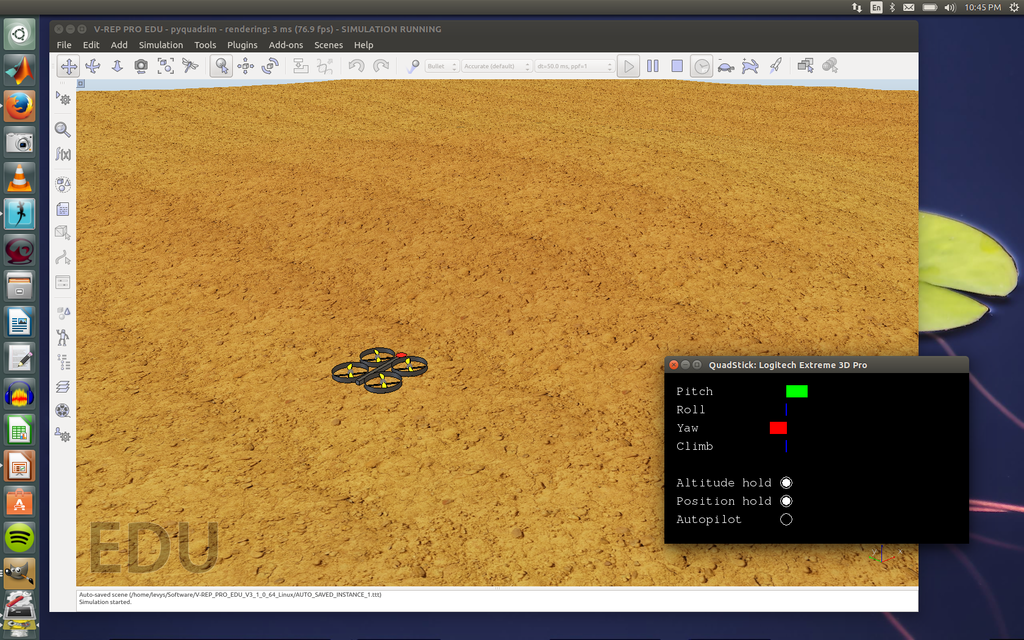
\includegraphics[width=0.75\linewidth]{img/pyquadsim}
	\label{fig:pyquadsim}
	\caption[Screenshot of the PyQuadSim project]{Screenshot of the PyQuadSim project. Source: \citep{pyquadsim}}.
\end{figure}
\pagebreak

\gls{unity} was chosen over alternatives for 2 reasons. Firstly, the company had experience with developing products using this engine. This opened up the opportunity for the company to do code reviews and generally being able to provide tips. Moreover, a realistic model for the drone and a variety of warehouse assets were available. The second and most important reason for choosing Unity, however, was \gls{mlagents}.

\section{Unity Simulation}
The original simulation can be seen in figure \ref{fig:first_sim}. It was made so each time the warehouse was generated, it would have a random size and amount of racks ranging from 1 to 8 racks. It was also equipped with an option to turn on or turn off training mode. Turning on training mode would minimize graphical load by replacing the models with simpler shapes and textures, as seen in the right image of figure \ref{fig:first_sim}.

\begin{figure}[h]
	\centering
	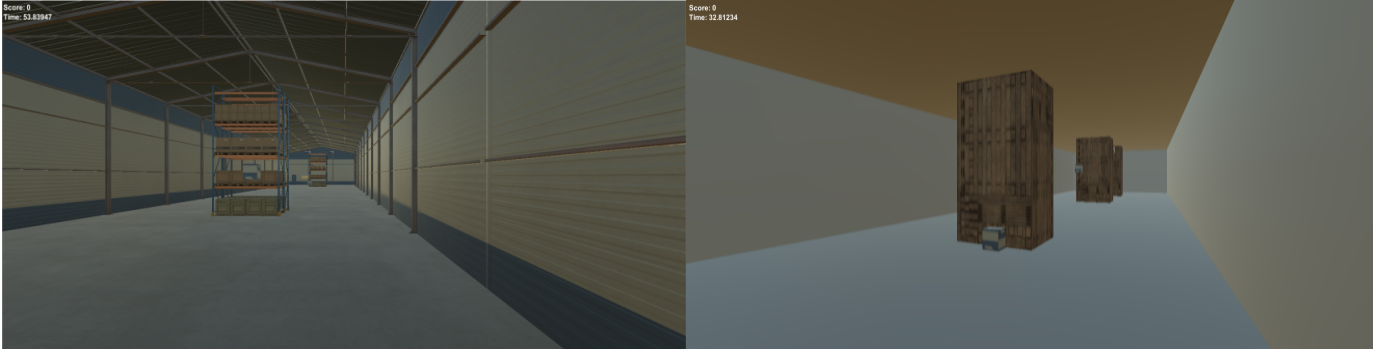
\includegraphics[width=\linewidth]{img/unity_real_training}
	\label{fig:first_sim}
	\caption{First design of the Unity warehouse simulation.}
\end{figure}

Based on feedback by the company the design was changed to feature 2 long rows of racks instead, as this was considered closer to the real situation. This was changed as displayed in figure \ref{fig:second_sim}, while maintaining the option for toggling training mode and a variable warehouse length. Both designs also featured targets spawning in at random positions in front of the racks. These targets functioned as an indication for where the drone should fly, and would grant the drone an increase in score whenever the drone flew over it. The simulation was made so that the view on screen simulated the view a real drone would have through its front-facing camera.

\begin{figure}[h]
	\centering
	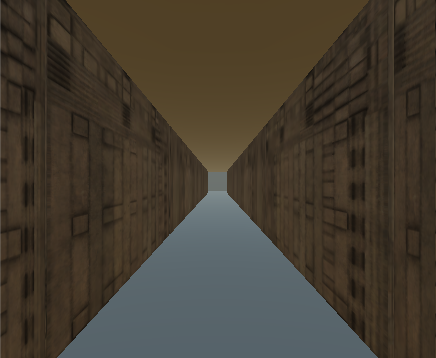
\includegraphics[width=0.5\linewidth]{img/sim_reinforcement}
	\label{fig:second_sim}
	\caption{Updated design of the simulation in training mode.}
\end{figure}

\section{ML-Agents Classes }
The implementation of the simulation with \gls{mlagents} contains 4 major parts: generator classes, the Unity package, the \gls{mlagents} package and its inheriting classes, and the class for reading a configuration file. Since the Unity package is the default package that all c\# Unity projects use, it will not be discussed here. A class diagram can be found in appendix \ref{app:sim_class_diagram}.

\paragraph{Generator} Generator is an abstract class that has concrete implementations for spawning the drone, warehouse, and the targets. Using the strategy design pattern, all the generators are registered and invoked by the DroneAcademy class.

\paragraph{DroneAcademy} DroneAcademy inherits from the Academy class within the ML-Agents package. It is responsible for all operations around the environment during training, for example destroying or adding new objects to the scene.

\paragraph{DroneAgent} DroneAgent inherits from the Agent class within the ML-Agents package. The object containing an implementation of the Agent class is meant to be controlled by a neural network (or "brain" in the context of Unity) during training.

\paragraph{ConfigHandler} ConfigHandler reads an external configuration file that contains information about how to generate the scene. Examples include the size of the warehouse and whether or not to enable training mode.

\section{Reinforcement Learning \& Imitation Learning}
For the \gls{RL} implementation the standard models provided by \gls{mlagents} were used. The \gls{RL} implementation was given the drone's coordinates, horizontal and vertical velocity, camera input, as well as the target's coordinates as input. The drone (or "agent" in \gls{RL} lingo) then was given 10-60 seconds (based on the warehouse size) to reach its target, and was rewarded based on its time left after reaching its goal. The agent was also mildly penalized for moving, in order to motivate it to keep its movement to a minimum. Once the agent had reached its target, the environment would reset and the warehouse would be regenerated using a random size, and the end of a so-called episode would then be reached. The ending of an episode means that the total reward score for that lifetime is finalized. In case the drone would crash into something, the episode would end immediately and the total reward score would be the lowest possible. Unfortunately, after having run several training sessions spanning somewhere between 10 minutes and 3 hours, the agent did not seem to learn. It kept flying a similar pattern, where it would fly up and slightly left or right, crashing into the ceiling. 
\\\\
As alternative, another model provided by \gls{mlagents} was used. This model, however, was for \gls{IL}. While they are both genetic algorithms, the major difference between \gls{IL} and \gls{RL} is that \gls{IL} does not make use of a predefined reward function. Instead, it tries to derive that function by imitating an expert (human) player. As a result, the simulation was slightly altered to spawn 2 identical warehouses that allowed for multiplayer (human vs. agent), as seen in figure \ref{fig:sim_imitation_scene_training}. To monitor progress, the simulation was altered to display both the view of the human-controlled drone and the agent-controlled drone in a split screen manner. This, however, also did not show any significant results. Even after having provided demonstrations for an hour, the agent kept moving slowly until it crashed in its nearest object, and did thus not show any sign of learning.
\begin{figure}[h]
	\centering
	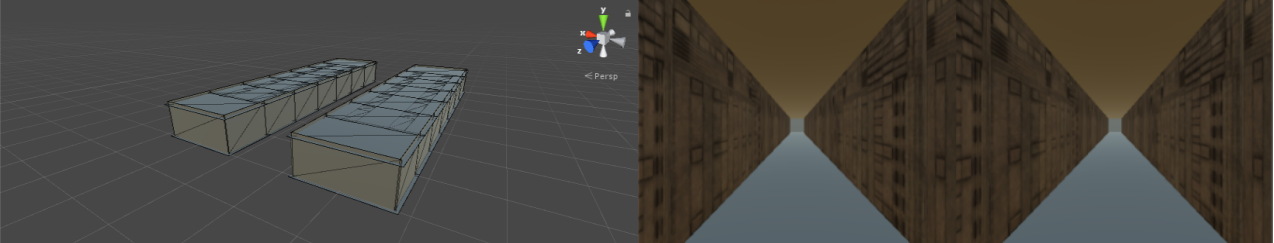
\includegraphics[width=\linewidth]{img/sim_imitation_scene_training}
	\label{fig:sim_imitation_scene_training}
	\caption[Simulation altered for running for imitation learning]{Simulation altered for running for imitation learning. The left image shows the warehouses from the outside, and the right image shows the view seen during training.}
\end{figure}

